\section{Application of Graphs}

\subsection{Structure of the Web}

The web can be treated as a directed graph where each link (url) is an edge pointing to another web page. Any directed graph can be broken down into $2$ components \texttt{(1)} \textit{Strongly connected component} where any node can reach any other node via a directed path \texttt{(2)} \textit{Directed acyclic graph, DAG} where if node $u$ can reach $v$, then $v$ cannot reach $u$.

Treating a strongly connected component (SCC) as one node, any graph can be ``distilled" into a directed acyclic graph (DAG), as shown below. Nodes $B, C, D, E$ form an SCC. Compressing these nodes into one $SCC$ node, we turned a ```mixed" graph into a DAG. Notice that there cannot be intercepting $SCC$s because any such intersection will force the $2$ SCCs to become a larger one due to definition of strongly connected component. 

{
\centering
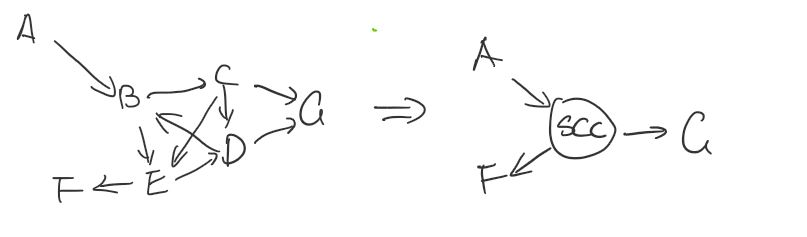
\includegraphics[width=0.75\textwidth]{notes/img/n3_scc.JPG} \par
}

As shown below, the famous bow-tie analogy for the structure of the web was proposed in 1999 \href{http://snap.stanford.edu/class/cs224w-readings/broder00bowtie.pdf}{[link]}. The graph was obtained after crawling through $203$ million URLs (web pages) and $1.466$ billion links. \texttt{IN} is a set of nodes that can reach \textit{SCC} whereas \texttt{OUT} are nodes that can be reached by nodes in \textit{SCC}. Other components are defined following similar convention.

{
\centering
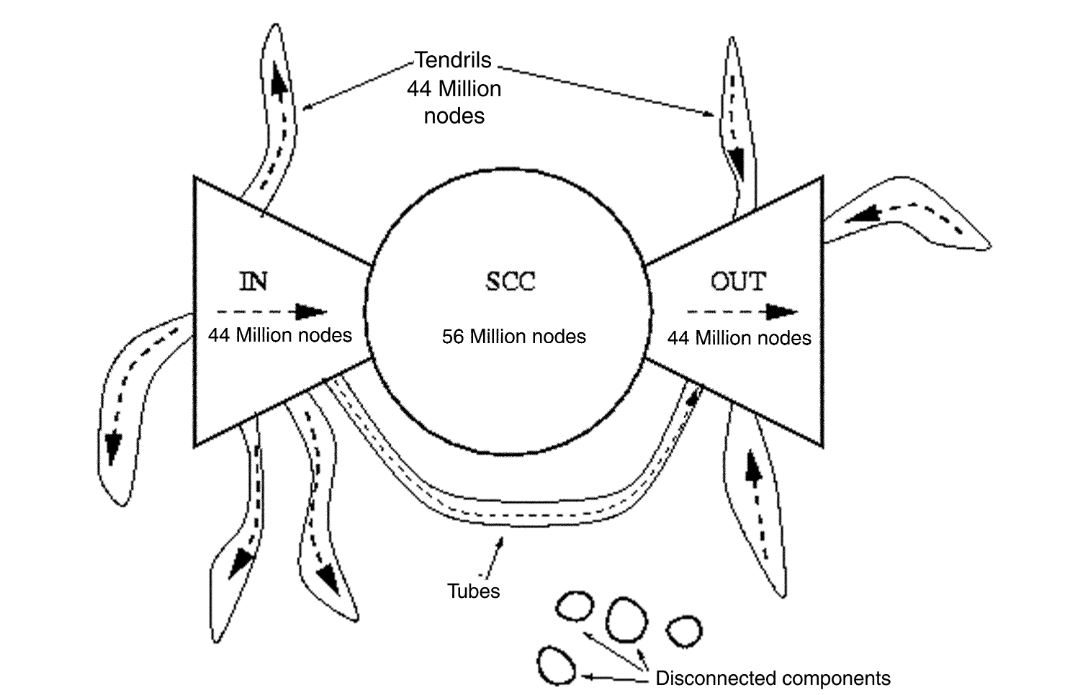
\includegraphics[width=0.7\textwidth]{notes/img/n3_web.JPG} \par
}


At a glance, you might be wondering how does one URL connect to a whole bunch of all other URLs? Well, the next image extracted from \textit{Networks, Crowds, and Markets: Reasoning about a Highly Connected World} \href{https://www.cs.cornell.edu/home/kleinber/networks-book/networks-book-ch13.pdf}{[link]} illustrates how such connection can happen for college admission. BTW, the craw was supported by \texttt{AltaVista} \href{https://en.wikipedia.org/wiki/AltaVista}{[link]}, world's first modern search engine and has since been absorbed into Yahoo! search (which then is no longer popular, \texttt{Yahoo.com} is only 10-th website on Alexa ranking).

{
\centering
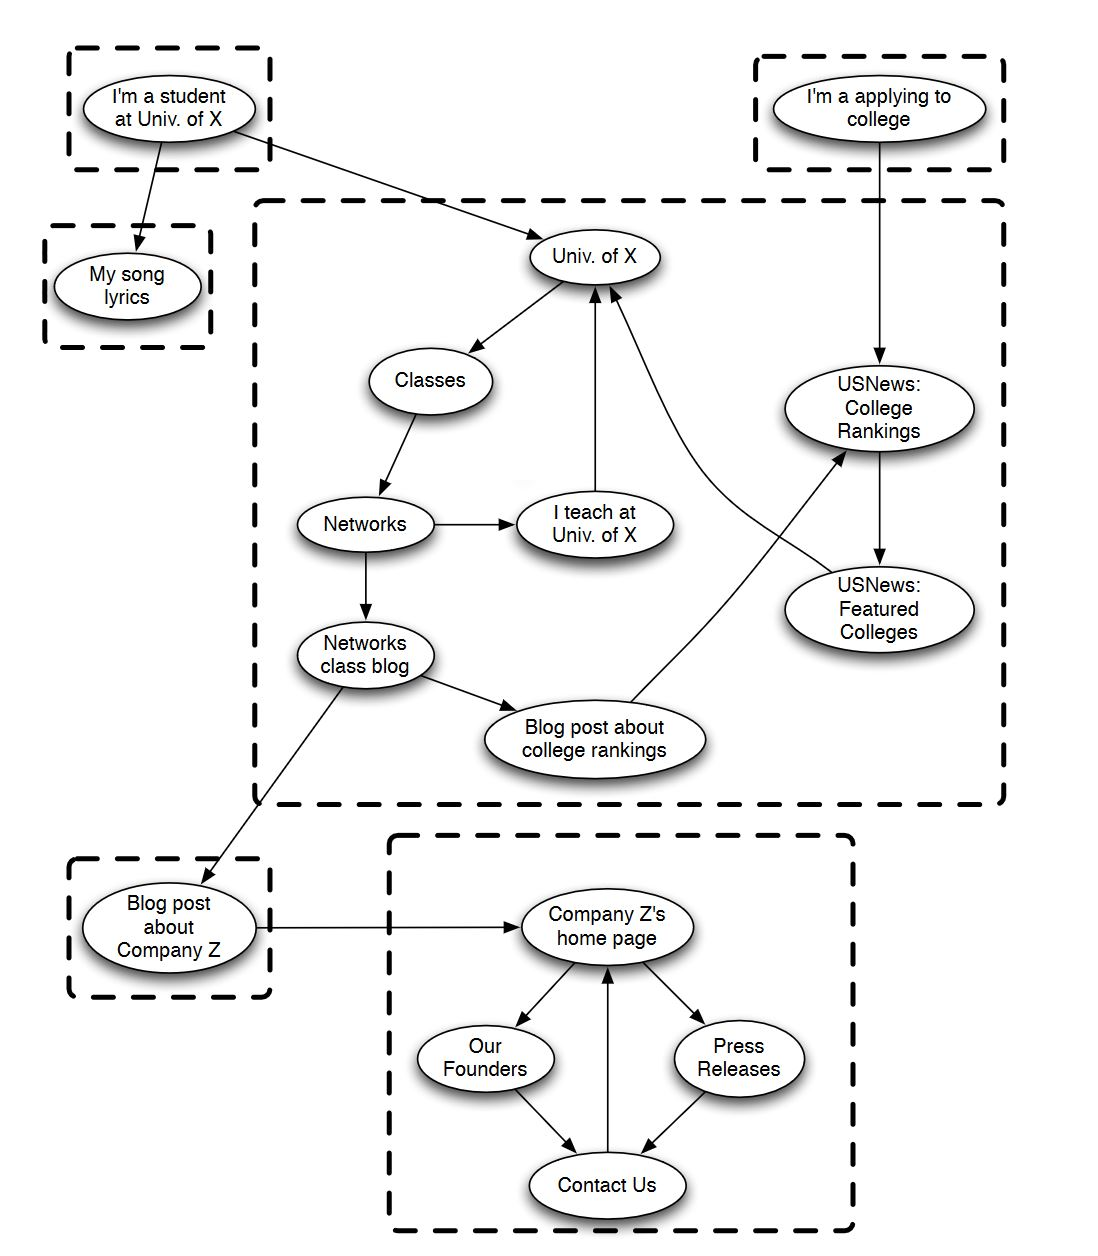
\includegraphics[width=0.75\textwidth]{notes/img/n3_scc_2.JPG} \par
}


To draw such bow-tie, we need to be able to classify each URL into \texttt{IN}, \texttt{OUT}, \texttt{SCC}, \texttt{Tendrils}, \texttt{Tubes} and \texttt{Disconnected components}. Using traditional search/traversal algorithms such as BFS and DFS, we can easily identify nodes reachable by node $v$ and nodes that reach $v$. Essentially, nodes reachable from $v$ from a tree rooted at $v$, let's call this $Out(v)$. Similarly, we can construct a ``reversed" tree for nodes that lead to $v$, let's call this $In(v)$. Clearly, an \textit{SCC} containing node $v$ is simply $Out(v) \cap In(v)$. With \textit{SCC}, \texttt{IN} consists of nodes ``reverse-reachable" by \texttt{SCC}. Tendrils originating from \texttt{IN} are nodes reachable by \texttt{IN} but not in \texttt{SCC} and not in \texttt{OUT}. Depending on the structure of this network, we might observe several and potentially sizable \texttt{Disconnected components}. 


Following only out-links, we can plot the following diagram. Most of the blue portion here represents \texttt{IN} while the pink portion represents \texttt{SCC} and \texttt{OUT}. Overlaying this with nodes reached through in-links (``reversed tree"), we can again see the proportion of nodes in \texttt{IN}, \texttt{SCC} and \texttt{OUT}. 

{
\centering
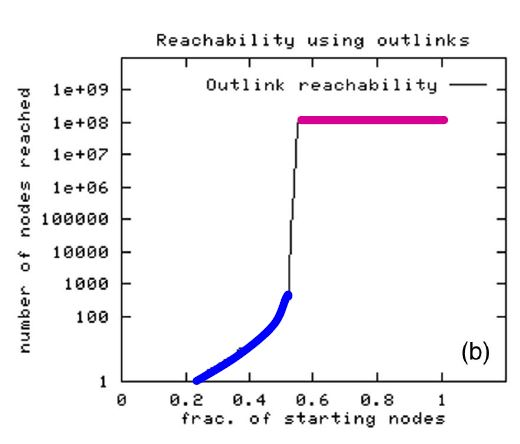
\includegraphics[width=0.55\textwidth]{notes/img/l11_p16_reachable.JPG} \par
}

Web is a bow-tie analogy is basesd on result obtained pre-2000. The \texttt{WWW} has evolved substantially since then (think how, as long as you point to Google, you point to the world). A report in the 2019 offering of \textit{CS 341} \href{https://web.stanford.edu/class/cs341/project/Kang_slides.pdf}{[link 1]}\href{https://web.stanford.edu/class/cs341/project/Kang_report.pdf}{[link 2]} shows that the current web looks more like a tie, where \texttt{IN} and \texttt{SCC} components have not changed substantially but a huge \texttt{OUT} portion has developed and is continuing to grow according to web crawls conducted in 2003, 2004 2007 and 2010. It might surprise you that \texttt{adobe.com} is a highly popular destination domain due to sites that tell you to download \textit{Adobe Reader}. \texttt{youtube.com} and \texttt{facebook.com} have moved up the rank to be come the most popular destination sites. We strongly suggest you to to read the report.

\subsection{PageRank}

Famously Google's success is based on its use of PageRank. As the name suggests, PageRank is a method of ranking importance of web pages. The basic idea behind PageRank is that pages with lots of in-links (those pointing to the page) is more important than one with few. For example \href{www.stanford.edu}{stanford.edu} has $23,400$ in-links while \href{www.joe-schmoe.com}{joe-schmoe.com} has $1$ in-link (WARNING! This site is not for the faint-hearted). Moreover, not all links carry equal importance. A site like \texttt{joe-schmoe.com} can setup lots of self-refernces or have a swarm of other sites point to it (link farm). Modern search engine optimization (SEO) techniques, including simple PageRank operations that we will discuss later, can filter out many forms of link farm.

PageRank follows a ``flow" model. That is, rank of nodes flow to children nodes. Therefore PageRank is an iterative process. As shown below, let $r_v$ represent the \textit{importance} of a node. Then node $i$ has $3$ out-links and node $j$ has $4$ out-links, therefore node $j$ carries $r_j = \frac{r_i}{3} + \frac{r_k}{4}$ important. It subsequently distributes $\frac{r_j}{3}$ to its own out-links.

{
\centering
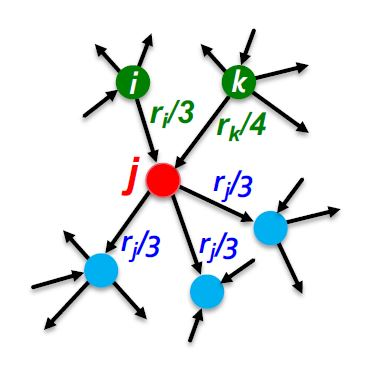
\includegraphics[width=0.4\textwidth]{notes/img/l11_p23_pagerank.JPG} \par
}

More mathematically, for node $j$ and its parents $P_j$, and $d_v$ as number of out-links of node $v$, we write

\begin{align}
    r_j &= \sum_{i \in P_j} \frac{r_i}{d_i}
\end{align}{}

In matrix form, where $M$ is stochastic adjacency matrix. (Typical adjacency matrix that represent connectivity has $row \rigtharrow col$, meaning that number of out-links are sum of entries of a row. The setup for PageRank is to avoid having to write $M^T$ all the time). Stochastic adjacency matrix stores $\frac{1}{d_j}$ for corresponding locations along its columns. That is, if node $j$ has $3$ out-links, the stochastic adjacency matrix should look like the following. 

{
\centering
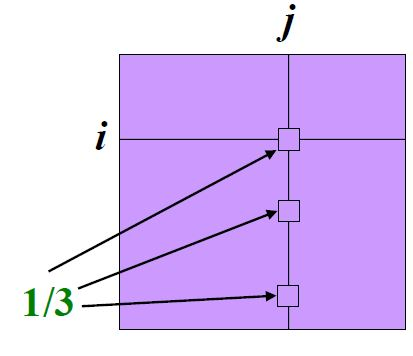
\includegraphics[width=0.4\textwidth]{notes/img/l11_p25_matrix.JPG} \par
}

With rank vector $r \in \mathcal{R}^{|N|}$ that represent rank for all nodes. For people familiar with Markov Chain, you should immediately recognize $M$ as state transition probability matrix where as $r$ is the state vector. See this note for basic note to Markov process \href{https://towardsdatascience.com/brief-introduction-to-markov-chains-2c8cab9c98ab}{[link]}. See CS168 notes \href{https://web.stanford.edu/class/cs168/l/l14.pdf}{[link]} for a slightly deeper explanation Markov Chain Monte Carlo and stationary distribution. See CS265 notes \href{https://theory.stanford.edu/~valiant/teaching/CS265/lectureNotes/l14.pdf}{[link]} \href{https://theory.stanford.edu/~valiant/teaching/CS265/lectureNotes/l15.pdf}{[link]} for more advanced topics. 

\begin{align}
    r^{new} &= M\cdot r^{old} \\
    r^{t} &= M^t \cdot r^{old} \text{\qquad superscript $t$ for matrix power} \\
    \forall r^{t}, \sum_{i}r_{i}^{t} = 1
\end{align}{}

Suppose that we have reached a stationary distribution, and $r_{final}$ represents such stationary distribution, that is $M^{t}u \rightarrow r_{final}$, where $t \rightarrow \infty$ and $u$ is any starting vector that represents a valid distribution ($\sum_{i} u_i = 1$). What we are getting at is, eventually we will have $r_{final} = M \cdot r_{final}$, therefore $r_{final}$ is an eigenvector of $M$ with corresponding eigenvalue of $1$.

Given the above, it is not hard to see the rationale behind the \textbf{power iteration method}, where

\begin{itemize}
    \item Initialize $r_{init}= [1/N, 1/N, \dots 1/N]^T$
    
    \item Iteratively compute $r_{(t+1)} = M\cdot r^t$
    
    \item Stop when $|r^{(t+1)} - r^t| < \epsilon$ for some pre-determined convergence threshold $\epsilon$
\end{itemize}{}

\paragraph{On stationary/limiting distribution and some formalities} While convergence is guaranteed for well-formed transition matrices (you should definitely read the CS265 note \href{https://theory.stanford.edu/~valiant/teaching/CS265/lectureNotes/l15.pdf}{[link]} for mixing time of Markov chains, also of course, you can treat this transition matrix as a random walk, which is the underlying Markov process. This Caltech note \href{http://www.math.caltech.edu/~2016-17/2term/ma003/Notes/Lecture15.pdf}{[link]} seems to be thorough as well with minor change in nomenclature), structures such as \textit{dead ends} and \textit{spider traps} can cause issues. Eventually these structures can siphon significant amount of importance from the overall network.

\begin{itemize}
    \item Dead ends. These are nodes with no out-links, so ``importance" accumulates here. In other words, importance given to the ``useful" part of the network decreases.
    
    \item Spider traps. These are self-referencing groups where out-links are only pointing to nodes within the group. 
\end{itemize}{} 

Let's formalize convergence of the \textit{power iteration method}. As said, we view transition matrix $M$ as transition matrix of a random walk performed on a \textit{Markov chain}. A Markov chain will reach a limiting distribution, that is, $S$ as all states (each state is a one-hot vector that can be represented by a single number, here it can simply be node $i$), $n$ as number of iterations, $X_i$ as the ``walker" being observed in state $i$ and $\pi_i$ as probability of the ``walker" being at node $i$,

\begin{align}
    \pi_j &= \lim_{n \rightarrow \infty} P(X_n = j) \qquad \forall j \in S
\end{align}{}

What the above means is that after a higher number of iterations, probability of landing at any node is the same as value in the limiting distribution $\pi_j$. Notice that $n\rightarrow \infty$ is necessary because the above is clearly not true for small $n$. With \textit{dead end}, limiting distribution will be one where the dead ends share some distribution while the remaining ``normal" nodes sharing no probability at all. With \textit{spider traps} the limiting distribution will not be unique. 

We then define stationary distribution, where the stationary distribution is solved rather than computed iteratively like the limiting distribution. For a Markov chain to have a unique stationary distribution, it must be 

\begin{itemize}
    \item Aperiodic. For all paths that the random walker can take to return to its starting position, lowest common divisor of length of these paths must be $1$. Typically, as soon as you see a sel-loop, the chain is aperiodic. 
    
    \item Irreducible. All nodes can reach any other nodes. Simply, no disconnected components, no ``one way" path to any component.
\end{itemize}{}

If the above are true then for transition matrix $M$, we are guaranteed to find $\pi = \pi M$ (or the transposed form, depending on definition of $M$) and $\sum_{j \in S}\pi_j = 1$. We claim that such stationary distribution IS the limiting distribution. Note that we do NOT know the number of steps needed to approach such distribution, we still have to bound the error by $\epsilon$.


%Before we get into handling \textit{dead end} and \textit{spider traps},


\paragraph{Google's solution} to spider-trap is through teleportation. Some background first, the paper was written by Sergei Brin and Larry Page in 1998 \href{http://ilpubs.stanford.edu:8090/422/1/1999-66.pdf}{[link]}. The proposed PageRank solution was tested on a $322$ million link database with $75$ million unique URLs  (Stanford Web Project \href{http://dbpubs.stanford.edu:8091/~testbed/doc2/WebBase/}{[link]}) and converged approximately $52$ iterations. By the way, 1998 was when Pentium II was running at less than \textit{half} of a gigahertz and your personal computer was running with $256MB$ of memory \href{https://www.ebay.com/itm/Vintage-Gateway-GP6-450-Pentium-II-450MHz-256MB-RAM-Desktop-Computer/133274714370?hash=item1f07cac102:g:~XwAAOSwB8Nd-Grg}{[ebay link]}. These computers are worse than the original Apple Watch \href{https://www.gsmarena.com/apple_watch_42mm_(1st_gen)-7696.php}{[link]}. Also, back then, ``Download Netscape Software" page had the highest importance (in case you don't know what Netscape is, see \href{https://en.wikipedia.org/wiki/Netscape_(web_browser)}{[link]}). 

Paraphrasing the paper, PageRank models a random surfer who randomly clicks through web pages. However, an actual web surfer can get bored, so the surfer might arbitrarily click to an unrelated page to restart this random walk, hence the ``teleportation". Suppose that at any time, the surfer has $1 - \beta$ probability of teleporting away. We can re-write the PageRank equation as 

\begin{align}
    r_j &= \sum_{i \in P_j } \beta \cdot \frac{r_i}{d_i} + (1 - \beta) \frac{1}{N} \\
    \intertext{\qquad \qquad Then in matrix form}
    r &= \beta \cdot M \cdot r + \frac{1 - \beta}{N} I \\
    r &= A \cdor r \text{\qquad where $A = \beta M + \frac{1 - \beta}{N} I$}
\end{align}{}

You might be wondering that there is a missing $r$ in the PageRank form. This is from the fact that $\sum_{i}r_i = 1$, so eventually the whole thing becomes adding a simple constant.

\paragraph{Dead end} ``leaks" PageRank because the rank goes to nowhere from the end node, causing sum of rows of $M$ or $A$ to be less than $1$. Therefore, $r^{new} < A_{dead\ end}r^{old}$. We can fill in the bank by either filling it up or by adding a shared constant. Due to potential size of the matrix, adding a shared constant is the more common approach, thus

\begin{align}
    r^{new} &= Ar^{old} \\
    r^{new'} &= r^{new} + \frac{1 - \sum_{i}r^{new}_i}{N} \text{\qquad add a simple constant}
\end{align}{}

\subsection{Topic-Specific PageRank}

A potential problem that can be solved using graphs is, given a bipartite graph representing a list of conferences and a list of authors, we want to know conferences that are the most similar to ICDM. Similar questions can be raised on, given a list of images and a list of boards (Pinterest), what are images that are the most similar to a select image. In the example below we want to use ``topic-specific" PageRank to find conferences that are the most similar to ICDM.

{
\centering
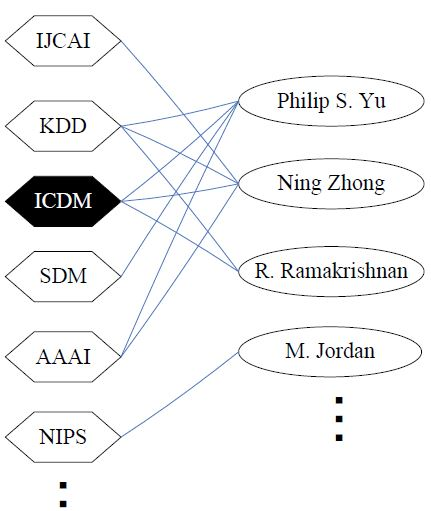
\includegraphics[width=0.4\textwidth]{notes/img/l11_p58_personalized.JPG} \par
}

Topic-specific PageRank is achieved by changing the teleportation part of PageRank. Instead of teleporting randomly to all nodes, only relevant nodes are allowed, called the teleport set. For this case, the teleport set is $\{ICDM\}$. Suppose we want to know things that are common to ICDM and KDD, the teleport set would then be $\{ICDM, KDD\}$. Recall the random walk equivalent for PageRank's transition matrix, with a pre-defined teleport set, topic-specific PageRank is simply a generalized form of random walk with restarts. Note that the proper ``random walk with restart" has teleport set size of exactly $1$ whereas a ``topic" can be represented by a larger teleport set.

The generalized topic-specific PageRank follows the same setup as PageRank but uses $\alpha$ as the probability for restart. 

\begin{itemize}
    \item \textbf{Vanilla PageRank} teleport uniformly at random to any node. All nodes have the same probability of being the target for teleportation.
    
    \item \textbf{Random Walk with Restarts} teleport to \textit{exactly} $1$ node. That $1$ node has probability of $1$ (teleportation vector being one-hot).
    
    \item \textbf{Topic-Specific PageRank} teleport to multiple nodes. However, these nodes can have different probabilities depending on definition of ``topic". 
\end{itemize}{}

Before we end here, it is worth noting that finding similar items through random walk and weighted random walk is one of the foundational tools for machine learning on graphs. See Section \ref{ss_4_graph_repr} for more details.


\subsection{Cascades}

Cascade is a fancy way of saying propagation. Originating from one node, we can build a directed propagation tree from a directed or an undirected network. Here, we use \textit{contagion} for the thing that is spreading (virus, fake news); \textit{infectious event} for the act of spread (adoption, infection, activation); \textit{main player} as the infected/active nodes. There are $2$ ways to model network cascade \texttt{(1)} deterministic, based directly on properties of nodes/edge \texttt{(2)} probabilistic, activation/infection is probabilistic.

% https://theory.stanford.edu/~valiant/teaching/CS265/ps4.pdf

{
\centering
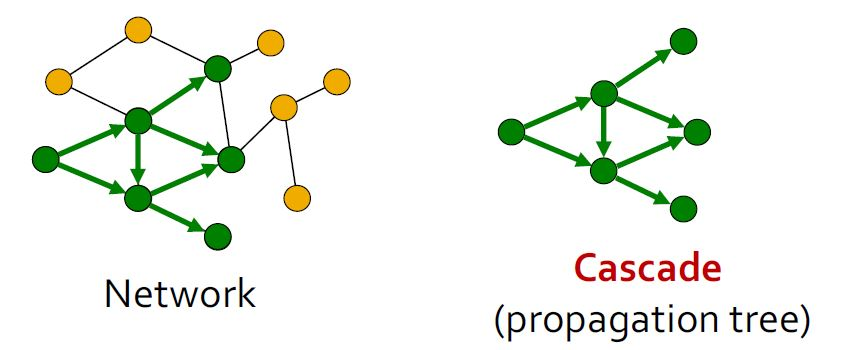
\includegraphics[width=0.75\textwidth]{notes/img/l12_p8_cascade.JPG} \par
}

\subsubsection{Decision based models}\label{ss_341_decision_based}

Decision based models are simple to implement and of course, deterministic in nature.

\paragraph{Software adoption} A simple examples is, in a friends network, people are adopting different video conferencing software. Suppose each person can only install either Skype (S) or Zoom (Z). We can define the payoff matrix as follows, where $a, b > 0$ for $2$ friends adopting the same software.

% Please add the following required packages to your document preamble:
% \usepackage{multirow}
\begin{table}[h]
\centering
\begin{tabular}{ll|ll}
                                              &   & \multicolumn{2}{l}{Friend 2} \\
                                              &   & Z             & S            \\\hline
\multicolumn{1}{c}{\multirow{2}{*}{Friend 1}} & Z & a             & 0            \\
\multicolumn{1}{c}{}                          & S & 0             & b           
\end{tabular}
\end{table}

Then for an undecided friend, we can compute the payoff of adopting $S \rightarrow r_S$ also $Z \rightarrow r_Z$. The friend adopts $S$ according to a threshold $t$, that is $\frac{r_S}{r_S + r_Z} > t$. Setting $t=0.5$ simply means $r_S > r_Z$.

For new software like Zoom, it is fair to assume that the entire network is initially populated with Skype users. Then marketing/financial incentive lets a number of early adopters flip to the Zoom camp, from which we can start iteratively decide whether Zoom will take over the network. Note that there can be an equilibrium state separated by some adoption boundaries. 

Similarly, suppose we allow adoption of both software. In the case where benefit of using both is larger than $a, b$, it is easy to see that more of both will be adopted. In contrast, if sharing has limited but non-zero benefit, only those along the adoption boundaries will be adopting both. Using example presented in class, we have the following payoff matrix, where $a, c$ are positive real number. The undecided friend is $W$ in $A - W - B$. 

\begin{table}[h]
\centering
\begin{tabular}{ll|ll}
                                              &   & \multicolumn{2}{l}{Friend 2} \\
                                              &   & A             & B            \\\hline
\multicolumn{1}{c}{\multirow{2}{*}{Friend 1}} & A & a             & a+1-c            \\
\multicolumn{1}{c}{}                          & B & a+1-c         & 1           
\end{tabular}
\end{table}

Then adoption by $W$ follows the following graph, essentially only adopting both when the harm $c < a + 1$ when $a$ is low and $c < 1$ then $a$ is high. This might be a little confusing because we have scaled $b$ to $1$. We'd have to plot a 3D graph by letting $b$ be arbitrary positive value. See 3D screenshot below (same color scheme), you can picture a 3-way division similar to the 2D image above it.

{
\centering
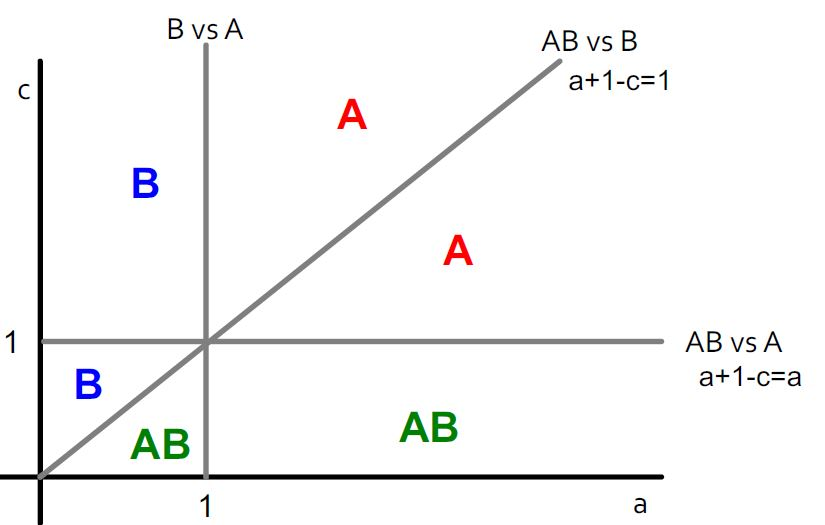
\includegraphics[width=0.6\textwidth]{notes/img/l12_p44_both.JPG} \par
}

{
\centering
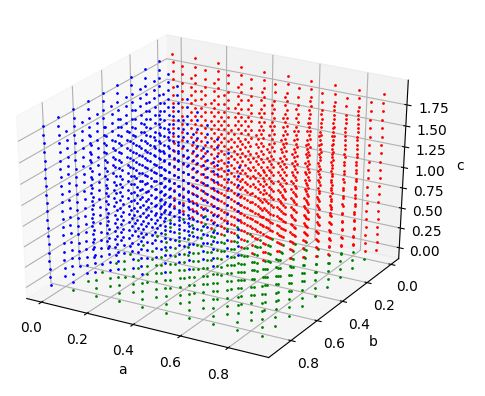
\includegraphics[width=0.6\textwidth]{notes/img/n3_both_2.JPG} \par
}

\paragraph{Protest and recruitment on social network} Example shown in class is about the anti-austerity 15-M protest in Spain (May 15-22, 2011 \href{https://en.wikipedia.org/wiki/Anti-austerity_movement_in_Spain}{[link]}). This is part of a series of ``Occupy" movements that include the famous 2011 Occupy Wall Street movement \href{https://en.wikipedia.org/wiki/Occupy_Wall_Street}{[link]}. 

In a research after the protest \href{https://arxiv.org/ftp/arxiv/papers/1111/1111.5595.pdf}{[link]} researchers identified 70 hashtags used by the protesters by crawling Twitter over a $1$ month period, yielding $581,750$ tweets from $87,569$ accounts. From here, researchers constructed \texttt{(1)} Full network with all follow as links \texttt{(2)} Symmetric network where only $a \leftrightarrow b$ following count as edges. Activation threshold is defined as $\frac{k_a}{k_{in}}$ where $k_a$ (number of active neighbours) and $k_in$ (total number of neighbours). This activation threshold is clearly dynamic and can be framed as ``social pressure". 

% As expected, social pressure is high at the beginning but as the movement gained momentum, when millions of Spaniards are on the street along with massive media coverage, social pressure dropped.

In the image below, there are $2$ peaks. \texttt{(1)} At low $\frac{k_a}{k_{in}}$, representing a large number of ``self-activating" users \texttt{(2)} At $\frac{k_a}{k_{in}} = 0.5$, a large portion of users joined the movement when more than half of the neighbours are active.

{
\centering
\includegraphics[width=0.55\textwidth]{notes/img/n3_15M.JPG} \par
}

The second image depends on $\Delta \frac{k_a}{k_{in}}$, that is, the speed at which their neighbours become active. Low threshold users become active regardless of the speed of change, but large threshold users only became active after a large burst of neighbourhood activation (2nd red dotted line). 

{
\centering
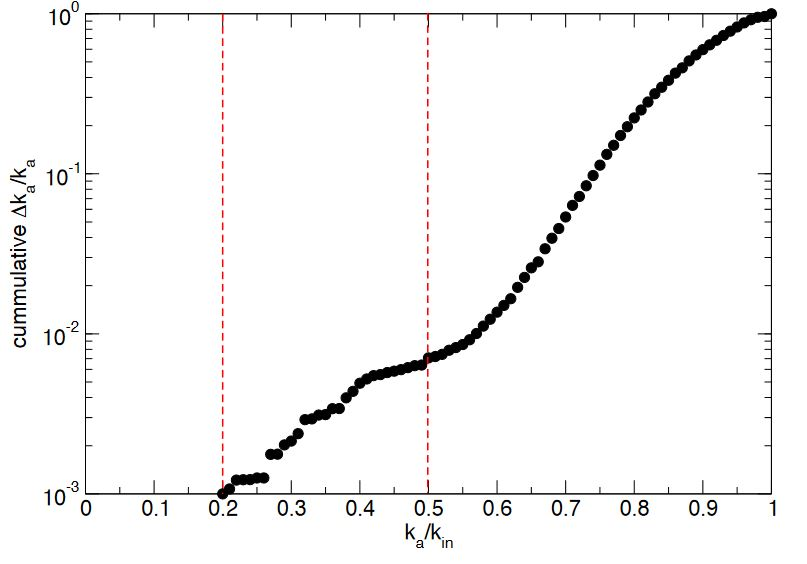
\includegraphics[width=0.55\textwidth]{notes/img/n3_cumulative.JPG} \par
}

The third image here compares size of a spreading ``core" against cascade size. What this is showing is that a larger initial core user will cause a more complete spread. Therefore to start a more influential campaign a large number of connected users need to be mobilized (for example, having game reviewing websites/popular streamers preview video game before launch then have them all tweet about this new game at the beginning). 

{
\centering
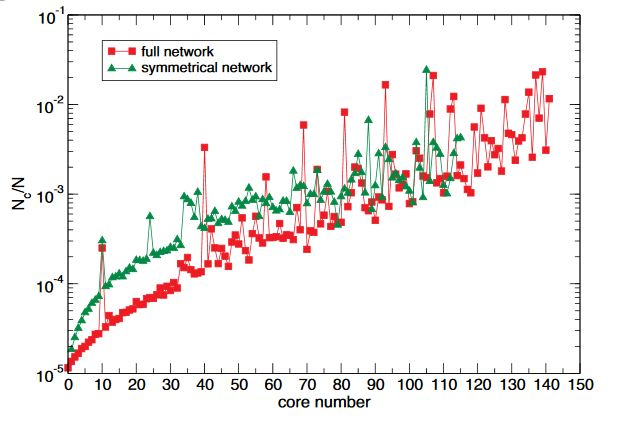
\includegraphics[width=0.5\textwidth]{notes/img/n3_core.JPG} \par
}

The following is extracted from \href{https://www.aclweb.org/anthology/D16-1191.pdf}{[link]}, where $k-core$ represents a connected subgraph where each node has at least degree $k$. Clearly, a cluster with high $k$ number is more central to the graph. We can obtain $k-core$ decomposition by repeatedly remove nodes with lower number of edges. Each layer removed represent one group of nodes with the same number of edges. 

{
\centering
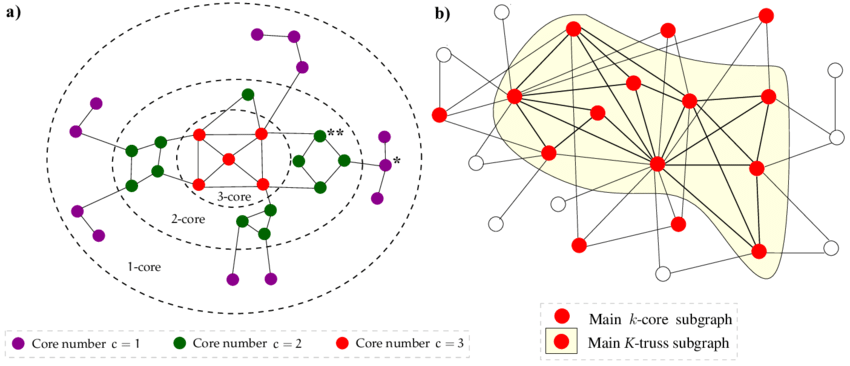
\includegraphics[width=0.75\textwidth]{notes/img/n3_kcore.png} \par
}

To summarize, if you want to start a campain on Twitter, you should be aware that 

\begin{itemize}
    \item Activation threshold for users is uniform, with exception of $2$ peaks at around $0$ (self-motivated) and around $0.5$ (more than half of neighbours)
    
    \item Most cascades are short (because you get out of the core area quickly on Twitter, remember the $3.7$ hops for average connection on Facebook)
    
    \item Successful cascades are started by central nodes (so you should consider arranging for a concerted tweet storm started by influencers/celebrities/review websites)
\end{itemize}{}

\subsubsection{Probabilistic models}

Clearly decision based models are not suitable for many real world applications. Simple rules are not suitable for complex scenarios such as spread of disease (depends on wearing protective equipment, method of contact, etc.) adoption of view (depends on your background, life event, etc.) and even installation of software (depends on cost, learning curve, capability of computer, etc.). Often it is much easier to model these complex properties with probability with frequent calibrations. 

The simplest representation of a probabilistic spreading model is a random tree. Starting at an active root, we want to know the number of people eventually activated, given that each edge has activation probability $q$ and each node is connected to $d$ leaves. With this, at each node, the probability of passing on the infection is 

\begin{align}
    p_{pass} &= 1 - (1 - q)^d   \text{\qquad $p_{not\ activated}=1-q$, then $d$ leaves}
\end{align}{}

We want to build a recurrent relationship into this equation, so instead of viewing the root of the $1 \rightarrow d$ nodes branch as having an active node, we let it having an $p^{(h)}$ chance of being active. Therefore, we can express

\begin{align}
    p_{pass}^{(h+1)} &= 1 - (1 - q \cdot p_{pass}^{(h)})^d
\end{align}{}

This interpretation does not care about the total number of nodes at each level, but instead view the parent as being a recurrent probabilistic parent, thus solving the problem of having to account for increasing number of nodes where each $d$ of such nodes are correlated to the parent (properly handling a growing Bayes's network is not fun). The the recurrent relationship is simply as shown.

\begin{align}
    f(x) &= 1 - (1 - q \cdot x)^d \\
    f(x=0) &= 0 \\
    f(x=1) &= 1 - (1 - q)^d < 1 \\ \\
    f^'(x) &= q\cdot d(1 - q \cdot x)^{(d - 1)} \\
    f^'(x=0) &= q \cdot d
\end{align}{}

Since all of $f'(x)$ are above $0$, $f(x)$ is monotonic and \textit{increasing} on $[0, 1]$. With some observation, it is not hard to tell that $f'(x)$ is monotonic (if you take the $2nd$ derivative) and \textit{decreasing} on $[0, 1]$. Let's plot a few $f(x)$ curve using a few $(q, d)$ tuples. Since the function starts from $f(x=1)$, observe direction of the arrows. All of these values approach the equilibrium value of $f(x)=x$. For the epidemic to die out, we must have $q \cdot d < 1$, then $lim_{h \rightarrow \infty}p^{(h)}=0$. This number, as you have heard on the news is called \textit{Basic reproduction number}, where $R_0 = q \cdot d$. For your reference, the 2020 COVID19 has estimated $R_0$ of $1.4 - 5.7$. Extracted from Wikipedia \href{https://en.wikipedia.org/wiki/Basic_reproduction_number}{[link]}, here is a few more data points. 

{
\centering
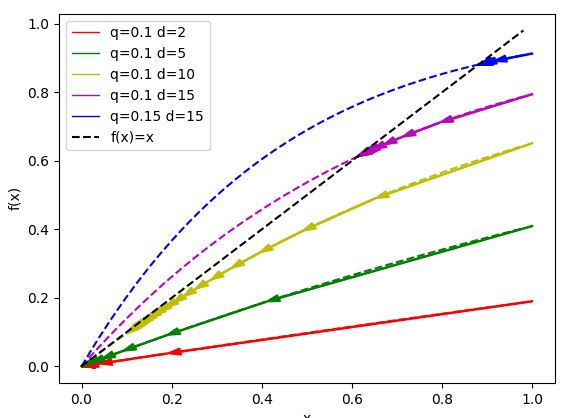
\includegraphics[width=0.55\textwidth]{notes/img/n3_prob_recursion.JPG} \par
}

\begin{table}[h]
\centering
\begin{tabular}{c|c|c}
\textbf{Disease}                & \textbf{Transmission} & \textbf{R0} \\\hline\hline
Measles                         & Airborne              & 12–18       \\
Chickenpox (varicella)          & Airborne              & 10–12       \\
Polio                           & Fecal–oral route      & 5–7         \\
Rubella                         & Airborne droplet      & 5–7         \\
Mumps                           & Airborne droplet      & 10–12       \\
Pertussis                       & Airborne droplet      & 5.5         \\
Smallpox                        & Airborne droplet      & 3.5–6       \\
COVID-19                        & Airborne droplet      & 1.4–5.7     \\
HIV/AIDS                        & Body fluids           & 2–5         \\
SARS                            & Airborne droplet      & 2–5         \\
Common cold                     & Airborne droplet      & 2–3         \\
Diphtheria                      & Saliva                & 1.7–4.3     \\
Influenza(1918 pandemic strain) & Airborne droplet      & 1.4–2.8     \\
Ebola(2014 Ebola outbreak)      & Body fluids           & 1.5–2.5     \\
Influenza(2009 pandemic strain) & Airborne droplet      & 1.4–1.6     \\
Influenza(seasonal strains)     & Airborne droplet      & 0.9–2.1     \\
MERS                            & Airborne droplet      & 0.3–0.8    
\end{tabular}
\end{table}

Clearly, as social distancing measures and protective equipment become widely adopted, $q, d$ changes, which is why disease control teams need to continuously sample the population to dynamically obtain accurate estimate of $q, d$ and change their models. The goal for disease control agency is to be sure that $R_0$ is below $1$ and remain at this level by enacting appropriate measures and encouraging disease limiting behaviour. The measures of course depend on disease transmission path

\begin{itemize}
    \item Droplets/particles in the air (flu, influenza): wearing mask/protective goggle, avoid direct contact, social distancing, etc.
    
    \item Contact and smear (herpes simplex, smallpox): avoid direct contact, especially around wound and/or mucous membranes
    
    \item Blood and tissue, direct and indirect via blood-sucking pests (AIDS, hepatitis, black death): avoid direct contact, hygiene of living environment, eradication of pests
    
    \item Contaminated water and food (salmonellosis, cholera): proper water sanitation and thoroughly cooking food/water
\end{itemize}{}

\paragraph{Flickr photo like propagation} The dataset consists of $100$ days of photo likes for $2$ million users, accumulating to $34,734,221$ likes on $11,267,320$ photos. 

The issue with estimating $R_0$ is that number of neighbours $d$ is not uniform across all users, so we estimate $R_0$ as the following ($d_i$ as degree of node $i$, $d$ as average node degree, $q$ as average proportion of neighbours infected). Then empirically, we can measure $R_0$ as proportion of directly infected nodes for the root noed of a cascade. 

\begin{align}
    R_0 &= q \cdot d \cdot \frac{avg(d_i)^2}{(avg\ d_i)^2}
\end{align}{}

As shown, the measured $R_0$ has high correlation with empirical $R_0$. The value is between $1$ and $190$, much higher than that of most contagious diseases. Moreover, in the next image, $2$ growth methods are compared. Photo $A$ is fueled by ``organic" growth from social network itself, whereas photo $B$ has external contributions at around day $40$, potentially due to the image being shared on an external website. 

{
\centering
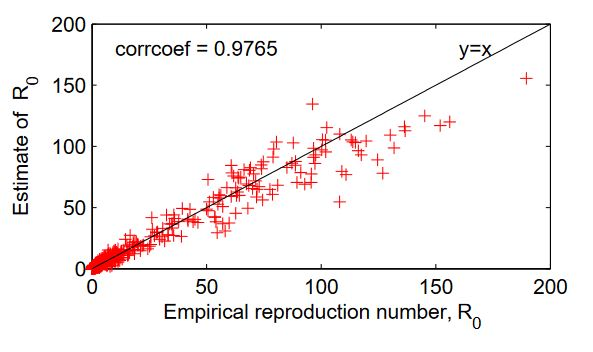
\includegraphics[width=0.55\textwidth]{notes/img/n3_flickr.JPG} \par
}

{
\centering
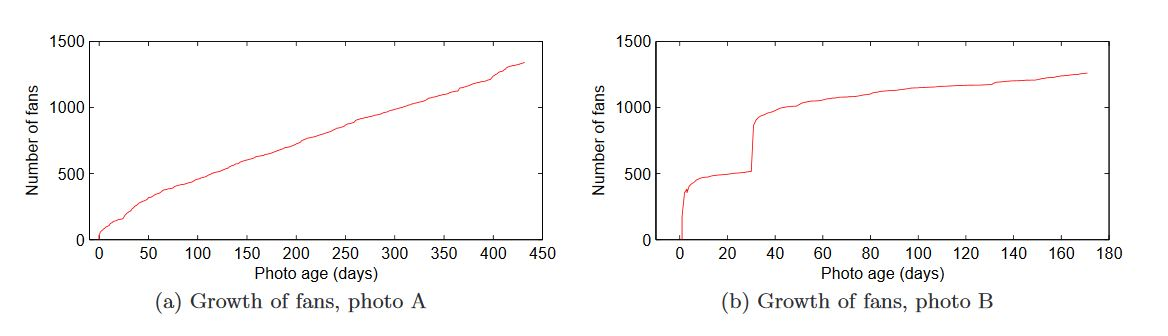
\includegraphics[width=1.0\textwidth]{notes/img/n3_flickr_2.JPG} \par
}

\subsubsection{Math driven epidemic model}

Diseases can also be modelled using a probabilistic model. However, the difficulty lies in correctly identifying social connections and modeling probability of spread. At the beginning of an epidemic, it is possible to trace those in contact by a pathogen carrier. As the epidemic develops, comprehensive tracking of contacts become near impossible, though modern tools such as GPS-capable smartphones and transparent yet privacy protecting data sharing software are utilized in the 2019-2020 COVID-19 outbreak. Epidemiologists resort to mathematical tools to model the spread, death and recovery of diseases.

\paragraph{Side note} For all of the following mathematical expressions, $S, I, R, E, Z$ represent proportions of population. The sum of these proportions should be $1$. On the Internet, you will see some versions including $N$, total population, thus $S, I, R, E, Z$ are number of individuals. Moreover, constants such as $\beta, \delta, \gamma$ can be a function of time as social distancing and advanced medical treatments start to take effect. 


\paragraph{SIR (susceptible, infected, recovered) model} This model is used for diseases which you become immune to after infection and death is rare, such as chickenpox. This model, as with all ``naive" math-based models, assumes perfect mixing. From a network perspective, the network is fully connected. The model can be expressed as 

\begin{align}
    Susceptible (S) &\rightarrow_{\beta} Infected (I) \\
    Infected (I) &\rightarrow_{\delta} Recovered (R) \\
    \frac{dS}{dt} &= -\beta SI \\
    \frac{dR}{dt} &= \delta I \\
    \frac{dI}{dt} &= \beta SI - \delta I
\end{align}{}

{
\centering
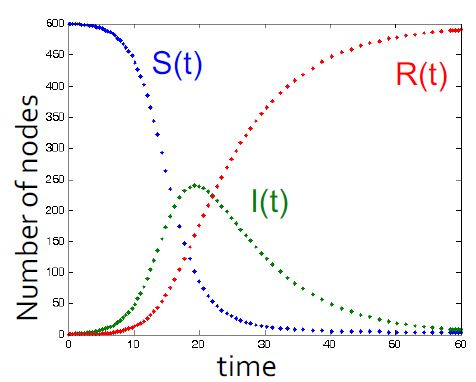
\includegraphics[width=0.5\textwidth]{notes/img/l13_p20_sir.JPG} \par
}

\paragraph{SIS (susceptible, infected, susceptible) model} This model is used for diseases which after cureved, the infected become susceptible again, such as fake news (you are convinced again) and e-coli. 
\begin{align}
    Susceptible (S) &\rightarrow_{\beta} Infected (I) \\
    Infected (I) &\rightarrow_{\delta} Susceptible (S) \\
    \frac{dS}{dt} &= -\beta SI + \delta I\\
    \frac{dI}{dt} &= \beta SI - \delta  I
\end{align}{}

{
\centering
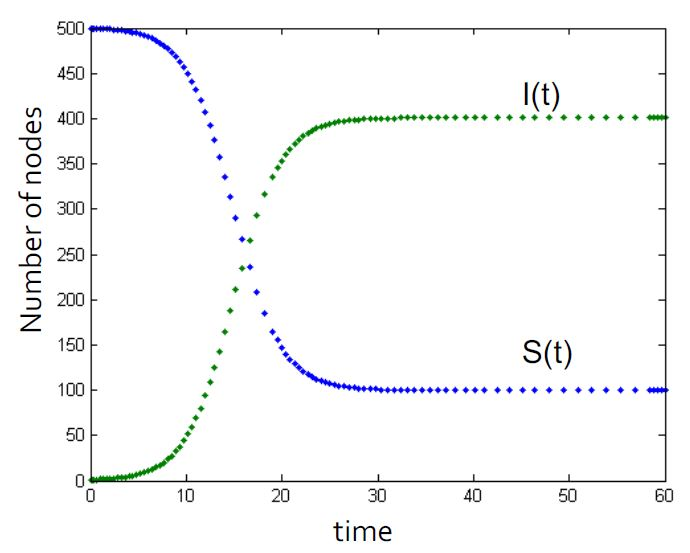
\includegraphics[width=0.5\textwidth]{notes/img/l13_p22_sis.JPG} \par
}

For this model we call $s = \frac{\beta}{\delta}$ as ``stregnth" of the spread. There certianly exists a threshold where if $s = \frac{\beta}{\delta} < \tau$ the disease will die out. We can show that if 

\begin{align}
    \frac{\beta}{\delta} &< \tau \\
                         &= \frac{1}{\lambda_{1, A}}
\end{align}{}

that is the threshold being the largest eigenvalue of the adjacency matrix, then the spread will die off. Recall that the largest eigenvalue $d_{avg} < \lambda_{1, A} < d_{max}$ (between average and largest node degrees). See more interpretations of eigenvalues of adjacency matrix \href{https://arxiv.org/pdf/1603.03960.pdf}{[here]} and \href{https://www.cs.yale.edu/homes/spielman/561/2012/lect03-12.pdf}{[here]}. In the graph below, ``autonomous system" simply means a system modeled by ordinary differential equations.

{
\centering
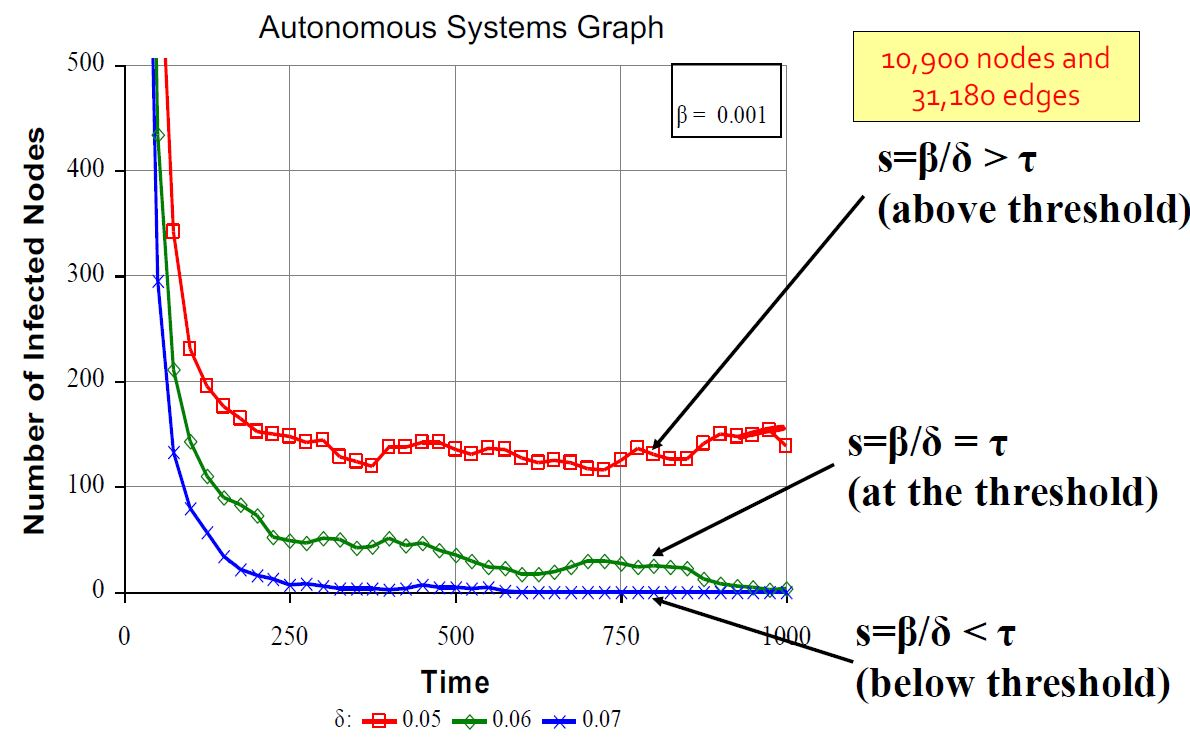
\includegraphics[width=0.7\textwidth]{notes/img/l13_p25_threshold.JPG} \par
}

Through simulation, we observe that \texttt{(1)} Below threshold, number of carriers decrease rapidly \texttt{(2)} Near threshold, number of carriers converge to $0$ \texttt{(3)} Above threshold, number of carrier stabilizes at above $0$.

{
\centering
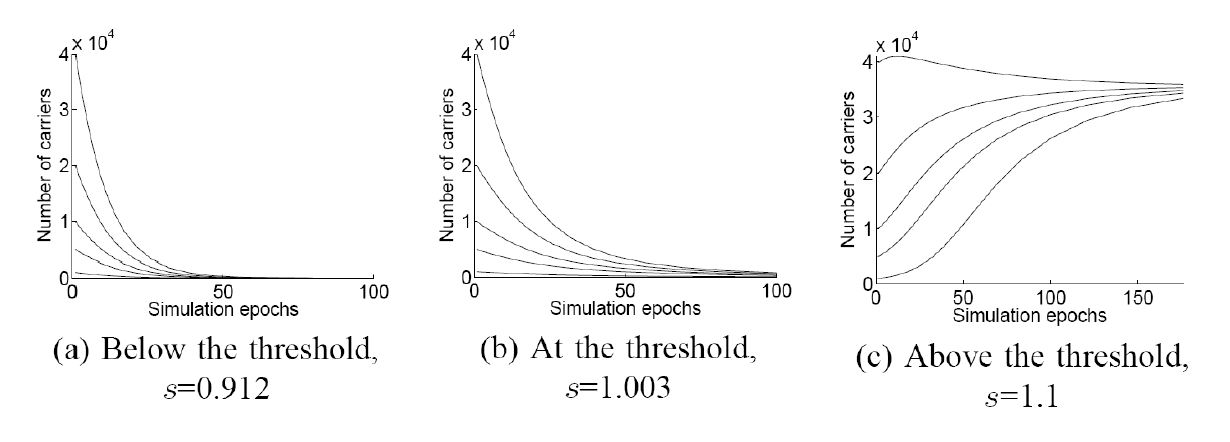
\includegraphics[width=1.0\textwidth]{notes/img/l13_p26_simulation.JPG} \par
}


\paragraph{SEIR (susceptible, exposed, infected, recovered) model} This model adds another stage to the \textit{SIR} model, where the \textit{exposed} stage can be seen as an incubation period. Worth noting that this is a period where the individual ins \textit{infected} but \textit{NOT infectious}, which is different from the incubation period of COVID-19, during which the individual is infectious. The following formulation is for SEIR, and $R_0$ for this formulation is still $\frac{\beta}{\delta}$, but can be more complex if latent period and duration of infectious period are accounted for \href{https://sites.me.ucsb.edu/~moehlis/APC514/tutorials/tutorial_seasonal/node4.html}{[link]}.

\begin{align}
    Susceptible (S) &\rightarrow_{\beta} Exposed (E) \\
    Exposed (E) &\rightarrow_{\alpha} Infected (I) \\
    Infected (I) &\rightarrow_{\delta} Recovered (R) \\
    \frac{dS}{dt} &= - \beta SI \\
    \frac{dE}{dt} &= \beta SI - \alpha E\\
    \frac{dI}{dt} &= \alpha E - \delta  I \\
\end{align}{}

Models that describe diseases in terms of stages are called compartmentalized models. Stages can have complex interactions with each other and each interaction leads to an additional ordinary differential equation. For the 2014 Ebola outbreak \ref{https://www.ncbi.nlm.nih.gov/pubmed/25642360}{[link]}, a more sophisticated version of \textit{SEIR model} was utilized, as shown below. Here, $H$ represents hospitalized cases, $F$ represents those who are dead but not yet buried; various $\gamma^{-1}$ represents duration of respective stage and $\alpha^{-1}$ being the incubation duration. This setup is to account for those not hospitalized and the fact that Ebola often transmitted through burial ceremonies and inadequate hospital quarantine measure.

{
\centering
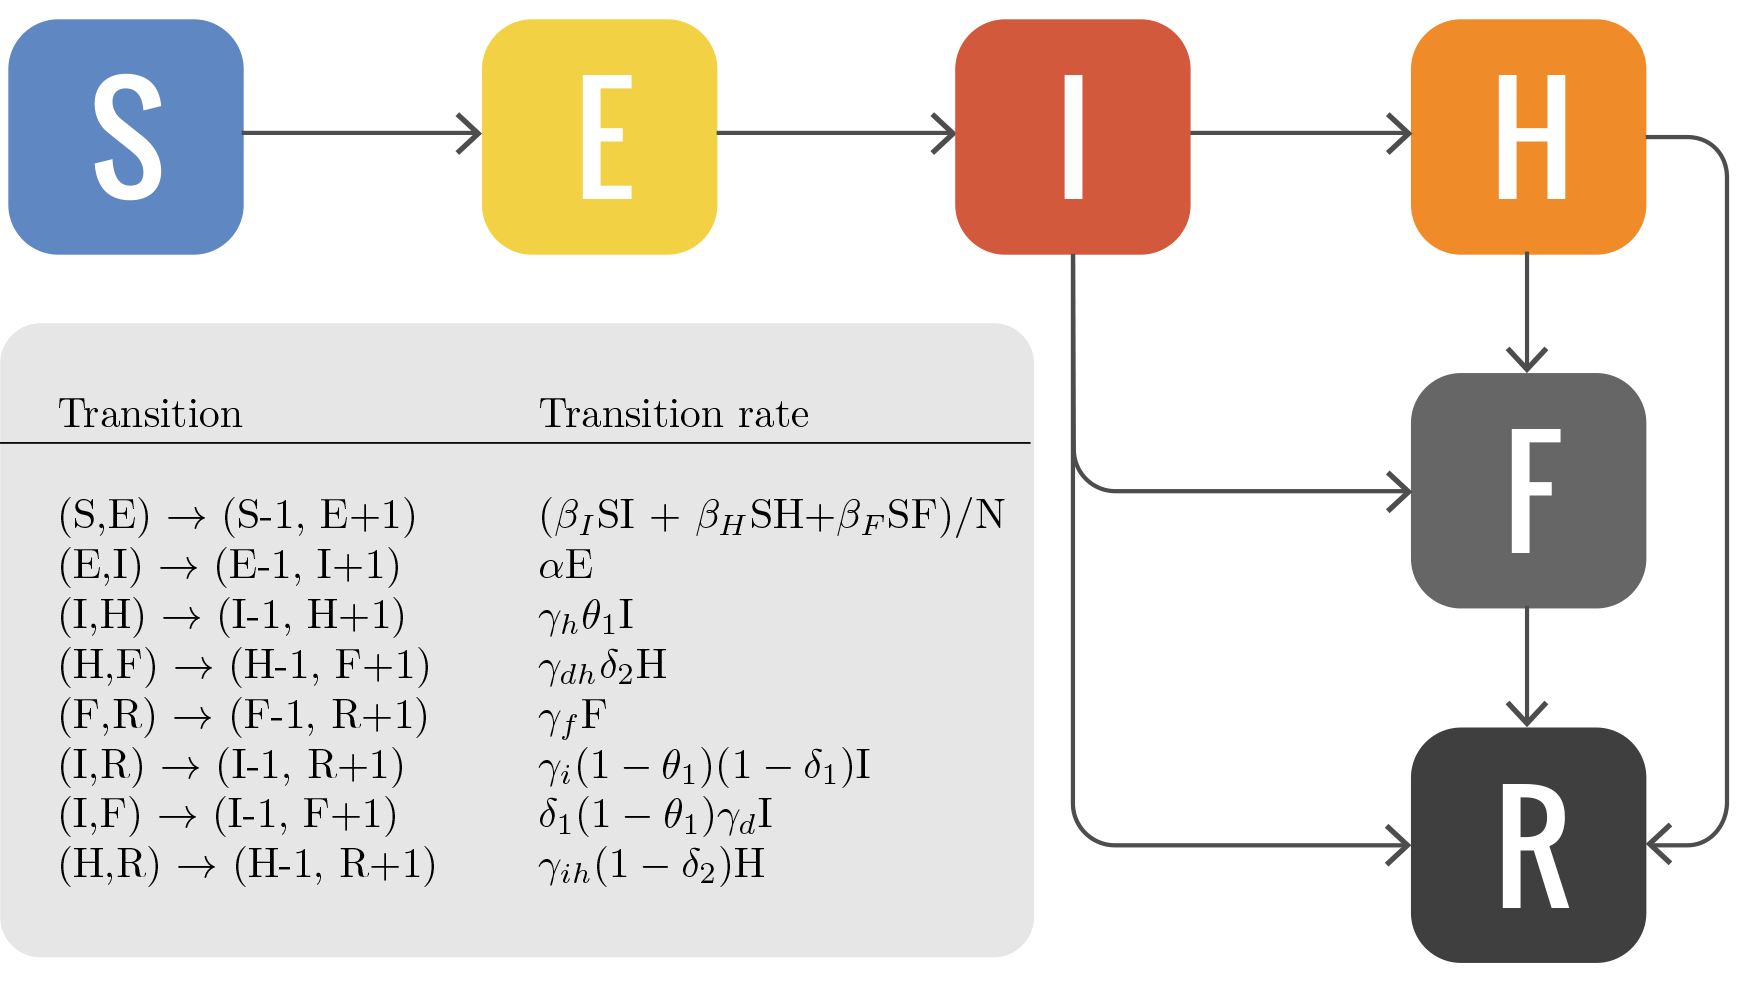
\includegraphics[width=0.95\textwidth]{notes/img/n3_ebola.png} \par
}

\paragraph{SEIZ (susceptible, exposed, infected, skeptical) model} This model \href{https://people.cs.vt.edu/naren/papers/news-rumor-epi-snakdd13.pdf}{[link]} claims to better represent the life cycle of rumor by replacing \textit{recovered} stage with \textit{skeptical} stage, meaning that the person become immune to being infected by fake news. The model has $2$ additional implicit transitory stages \texttt{(1)} upon receiving fake news and believing it, decides whether to re-post immediately or wait a few days \texttt{(2)} upon receiving fake news, decides to become skeptical or repost in a few days. \textit{Personally, since $E$ represents a stage of contemplation, we believe it is missing a $E \rightarrow Z$ transition that allows for a period of fact-checking instead of simply delaying the re-post. This additional link does complicate the ODE, which could be why the authors chose to leave it out}. 

{
\centering
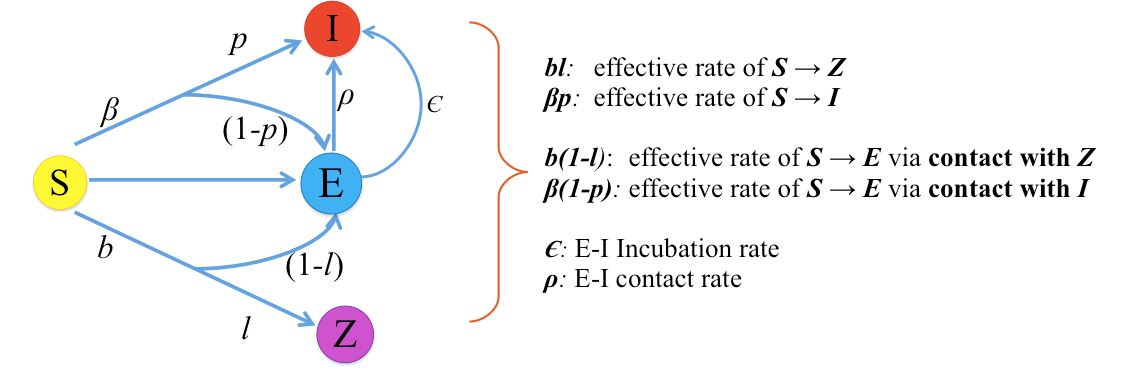
\includegraphics[width=0.95\textwidth]{notes/img/n3_seiz.jpg} \par
}

Mathematically, we have the following (leaving out all division by $N$ to be consistent with out previous expressions).

\begin{align}
    \frac{dS}{dt} &= - \beta SI - bSZ\\
    \frac{dE}{dt} &= (1-p)\beta SI + (1-l)bSZ - \rho EI - \epsilon E\\
    \frac{dI}{dt} &= p\beta S I + \rho E I + \epsilon E \\
    \frac{dZ}{dt} &= lbSZ \\
\end{align}{}

The observable part of this model is number of tweets sent by users, corresponding to an increase in number of infected people. Therefore, we want to optimize parameters to minimize $|I(t) - tweets(t)|$. The auhtors also defined a new parameter $R_{SI} = \frac{(1-p)\beta + (1-l)b}{\rho + \epsilon}$ to characterize spread of information on Twitter. The image below compares $R_{SI}$ for various events. Here, high $R_{SI}$ value represent ``convincing" information because $R_{SI}$ partially represents conversion rate, in contrast, rumors have much lower $R_{SI}$ due to their dubious nature that get people question their validity.

{
\centering
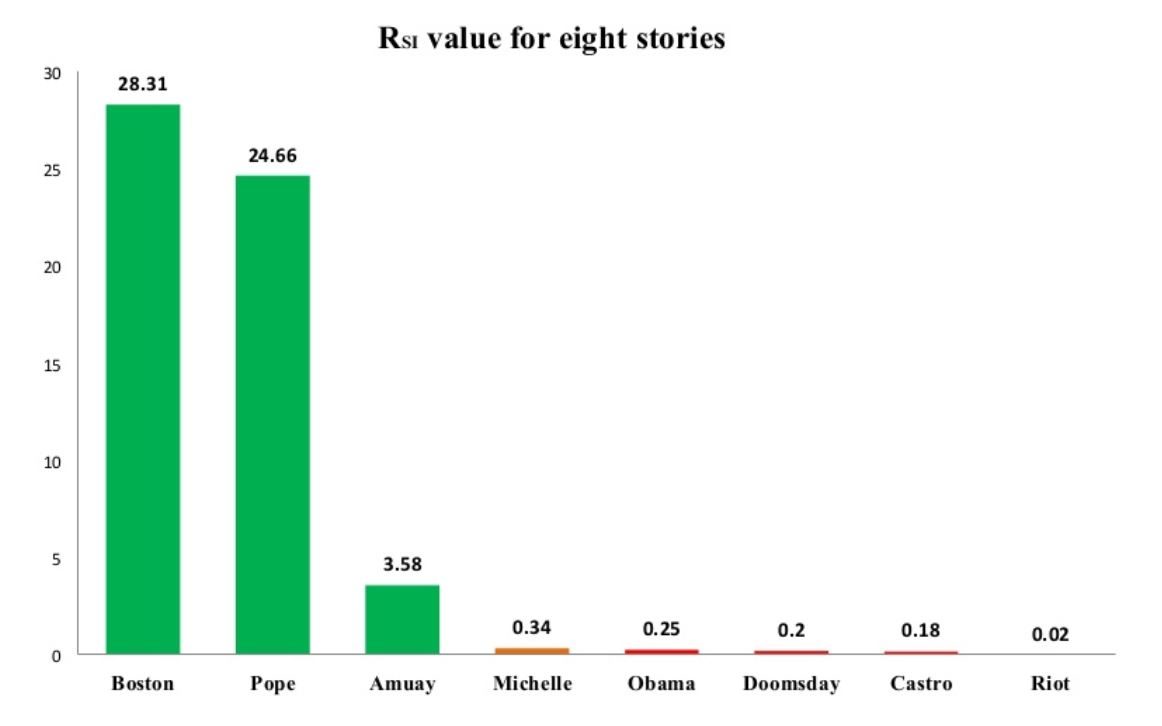
\includegraphics[width=0.75\textwidth]{notes/img/n3_seiz_compare.jpg} \par
}

\paragraph{Other compartmental models} We will not go in details for other models. However, compartments, or stages are used for more complex models.

\begin{itemize}
    \item \textit{Carrier (C)}. A stage in which a person carries the disease but suffer little to no symptom. In this stage, the person is infectious, unlike the \textit{exposed} stage in \textit{SEIR}. Models that include this stage is useful for diseases with length incubation AND infectious period. 
    
    \item \textit{Passive immunity (M)}. A stage in which a person has passive immunity. During this stage, the person carries insufficient amount (through breast milk or umbilical cord) or has yet to synthesize (immediately after vaccination) antibody. As you might have guesses, this stage is found in models for AIDS. 
    
    \item \textit{Temporary immunity (also R)}. A stage in which a person is temporarily immune to the disease, typical use case can be the seasonal flu.
    
    \item \textit{Deceased (D)}. A stage in which a person has died from the disease. Complimentary to this stage is typically a recovered stage. Essentially the $2$ outcomes for such disease is either death or permanent immunity. This is often used for particularly deadly diseases such as smallpox. 
\end{itemize}{}

\subsubsection{Independent cascade model}

An independent cascade model is one that has full control over all edges of the network, where each edge represents an activation probability $p_{uv}$. As said before, a fully connected network in which all edges have the same activation probability is the same as the mathematical models we discussed just now. The difficulty is that modeling a network full, potentially $O(n^2)$ number of parameters is quite difficult and susceptible to overfitting to limited data (Hopefully outbreak for the same disease happens once in a life time. Also, our society changes rapidly, we might have a functioning world government next time).

To alleviate this issue, we return to the decision based model (Section \ref{ss_341_decision_based}). We use the proportion of friends who are activated as basis for activation, then apply an activation function. This is called an exposure curve. Total number of adoptions can then form an adoption curve.

{
\centering
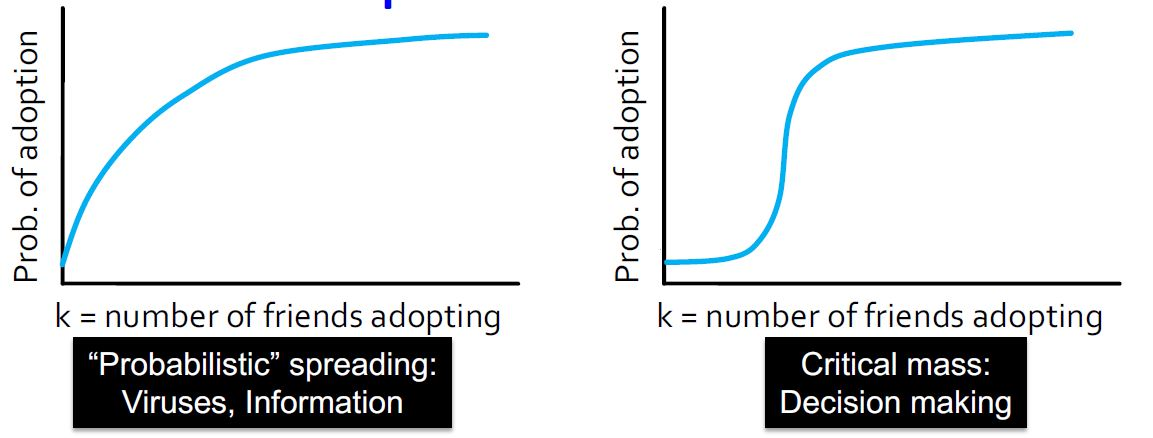
\includegraphics[width=0.95\textwidth]{notes/img/l13_p44_exposure.JPG} \par
}

{
\centering
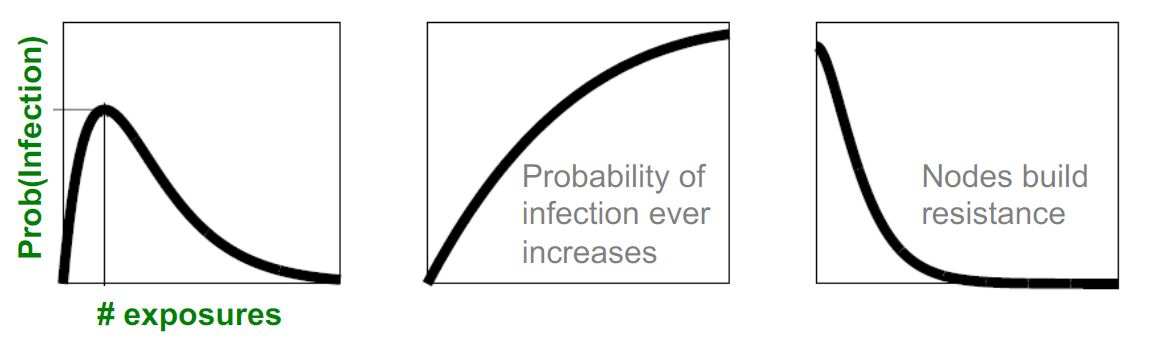
\includegraphics[width=0.95\textwidth]{notes/img/l13_p45_adoption.JPG} \par
}

As an example, back in early 2000s (June 2001 to May 2003), person to person recommendation of items via email was still a thing, \href{https://cs.stanford.edu/people/jure/pubs/viral-tweb.pdf}{[link]}, we were able to conclude from $8.2$ million observations related to DVD recommendations that the probability of purchasing saturated near $5\% - 6\%$. Similar behavior of the exposure curve can be observed for LiveJournal (some Russian blogging website) group membership \href{https://www.cs.cornell.edu/~lars/kdd06-comm.pdf}{[link]}, saturating at around $2\%$. Then in a 2011 paper \href{http://ra.ethz.ch/CDstore/www2011/companion/p113.pdf}{[link to free version, Springer needed for complete version]}, the exposure curve reaches peak quickly, but decrease until stabilization. We could potentially explain this as a transition from ``I want my friends to know" to ``many of my friends know this already". We can define the peak probability as \textit{stickiness} of a hashtag. We can also define the persistence as area under the exposure curve (with appropriate scaling and truncation of the x-axis). The study found that idioms and music have lower stickiness while sports and politics have higher stickiness compared to a randomly selected bag of hashtags.

{
\centering
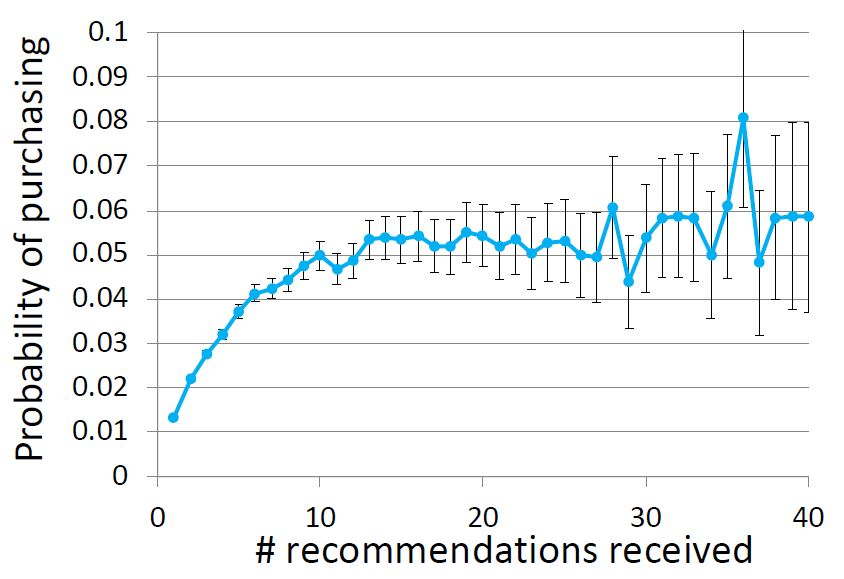
\includegraphics[width=0.95\textwidth]{notes/img/l13_p47_dvd.JPG} \par
}

{
\centering
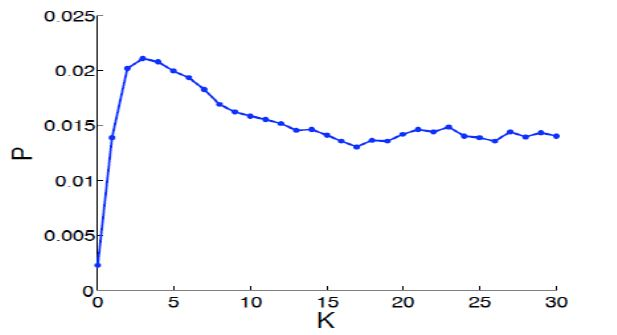
\includegraphics[width=0.95\textwidth]{notes/img/l13_p50_twitter.JPG} \par
}
